
\centering

\hypertarget{lista-de-exercuxedcios-sobre-fundamentos-de-sistemas-scada}{%
\subsection{Lista de Exercícios sobre Fundamentos de Sistemas
SCADA}\label{lista-de-exercuxedcios-sobre-fundamentos-de-sistemas-scada}}


\begin{enumerate}
\def\labelenumi{\arabic{enumi}.}
\item
  Quais os quatro níveis de automação relacionados à proteção e controle
  de subestações de energia elétrica, tendo em vista a possibilidade de
  monitoramento remoto e integrado de um conjunto de subestações?
  Comente sobre cada um dos níveis.
\item
  Com base na resposta do item anterior, descreva como a abertura de um
  disjuntor pode ser realizada em cada um dos níveis de automação de uma
  subestação. Descreva também como a atualização do estado do disjuntor
  é propagada em cada desses níveis via função de supervisão desse mesmo
  sistema.
\item
  Quais as tecnologias empregadas pelos relés de proteção desde sua
  concepção no início do século XX até os desenvolvimentos mais atuais?
  Descreva as principais características de cada uma.
\item
  De quando data o primeiro protótipo de sistema de supervisão e
  controle de processos industriais? Descreva suscitamente os principais
  avanços até os dias de hoje.
\item
  O que são as UTRs? Quais suas funcionalidades? Por que foram tão
  utilizadas na era dos relés eletromecânicos? Por que caíram em desuso?
  Em que situações ainda podem ser úteis? Qual sua principal diferença
  em relação aos modernos IEDs de proteção e controle?
\item
  Comente suscitamente sobre os principais protolcolos de automação
  utilizados no ambiente de subestações. A saber modbus, DNP 3.0, IEC
  101, IEC 104, MMS, GOOSE e Sampled Values.
\item
  Cite 5 exemplos de pontos digitais que devem ser monitorados pelo
  sistema SCADA de uma SE. Especifique o equipamento a que cada ponto
  está associado e contextualize sua funcionalidade.
\item
  Cite 5 exemplos de pontos analógicos que devem ser monitorados pelo
  sistema SCADA de uma SE. Especifique o equipamento a que cada ponto
  está associado e contextualize sua funcionalidade.
\item
  O que é uma Merge Unit? Para que serve? Por que vem sendo tão
  comentada nos últimos anos?
\item
  Quais os principais protocolos especificados pela norma IEC 61850?
  Qual a funcionalidade de cada protocolo citado?
\item
  Qual a definição de Sistema SCADA (\emph{Supervisory Control and Data
  Acsition System})? Quais os principais elementos desse tipo de
  sistema? Comente sobre cada uma delas.
\item
  Sobre os sinais analógicos, qual o padrão mais estabelecido para
  trasmissão desses sinais dos equipamentos de campo para os IEDs de
  proteção e controle? Especifique sua resposta em relação aos
  transformadores de instrumentos (TCs e TPs) e em relação às grandezas
  secundárias como temperatura, pressão, nível de líquidos, etc.
\item
  Comente sobre cada um dos processos descritos na figura abaixo:
\end{enumerate}

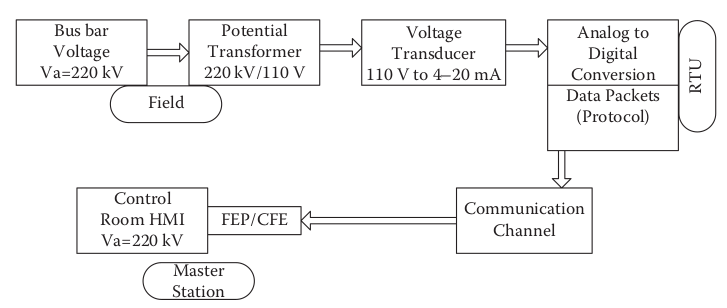
\includegraphics[width=0.8\textwidth,height=\textheight]{Figuras/fig1.png}


\begin{enumerate}
\def\labelenumi{\arabic{enumi}.}
\setcounter{enumi}{12}
\item
  Comente sobre a importância do sincronismo de tempo entre os
  disposisitivos de proteção e controle de uma subestação. Quais os
  principais protocolos utilizados para esse fim?
\item
  Quais as duas principais técnicas de coleta de dados entre os
  equipamentos supervisionados e os IEDs de proteção e controle?
  Mencione em sua resposta as vantagens e desvantagens de cada uma.
\item
  Comente sobre cada uma das funcionalidades de um IED de proteção e
  controle mostradas na figura abaixo:
\end{enumerate}

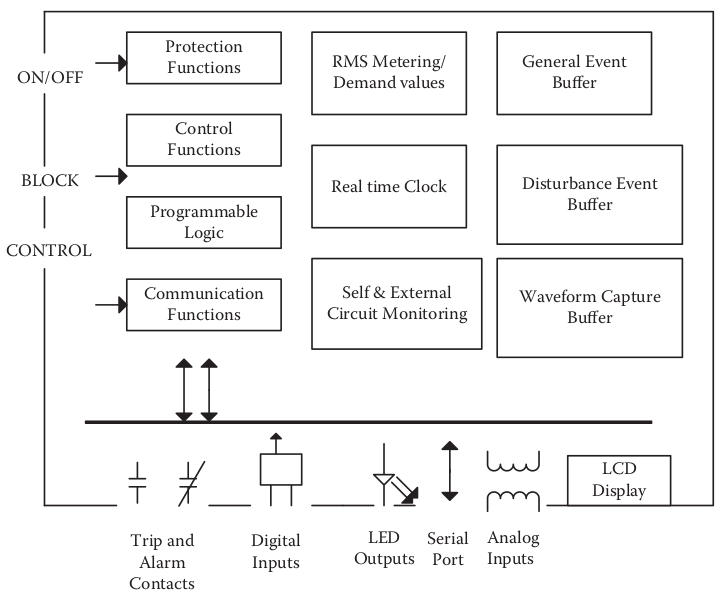
\includegraphics[width=0.8\textwidth,height=\textheight]{Figuras/fig2.png}

\hypertarget{lista-de-exercuxedcios-sobre-protocolos-de-rede-de-camada-de-enlace}{%
\subsection{Lista de Exercícios sobre Protocolos de Rede de Camada de
Enlace}\label{lista-de-exercuxedcios-sobre-protocolos-de-rede-de-camada-de-enlace}}

\begin{enumerate}
\def\labelenumi{\arabic{enumi}.}
\item
  Quais são alguns dos serviços possíveis que um protocolo da camada de
  enlace pode oferecer à camada de rede? Quais desses serviços da camada
  de enlace têm serviços correspondentes em IP? E em TCP?
\item
  Suponha que dois nós comecem a transmitir ao mesmo tempo um pacote de
  comprimento L em um canal de transmissão de taxa R. Denote o atraso de
  propagação entre os dois nós como \(d_{prop}\). Haverá uma colisão se
  \(d_{prop} < L/R\)? Por que sim ou por que não?
\item
  Qual é o tamanho do espaço de endereços MAC? E do espaço de endereço
  IPv4? E do espaço de endereço IPv6?
\item
  Suponha que os nós A, B e C se conectem à mesma LAN de broadcast (por
  meio de seus adaptadores). Se A enviar milhares de datagramas IP para
  B com cada quadro de encapsulamento endereçado ao endereço MAC de B, o
  adaptador de C processará esses quadros? Se sim, o adaptador de C
  passará os datagramas IP nesses quadros para a camada de rede C? Como
  suas respostas mudariam se A enviasse quadros com o endereço MAC de
  broadcast?
\item
  Por que uma consulta ARP é enviada dentro de um quadro de broadcast?
  Por que uma resposta ARP é enviada dentro de um quadro com um endereço
  MAC de destino específico?
\item
  Compare as estruturas de quadro para as especificações Ethernet
  10BASE-T, 100BASE-T e Gigabit Ethernet. Como elas diferem?
\item
  Considere três LANs interconectadas por dois roteadores, conforme
  mostrado na Figura:
\end{enumerate}

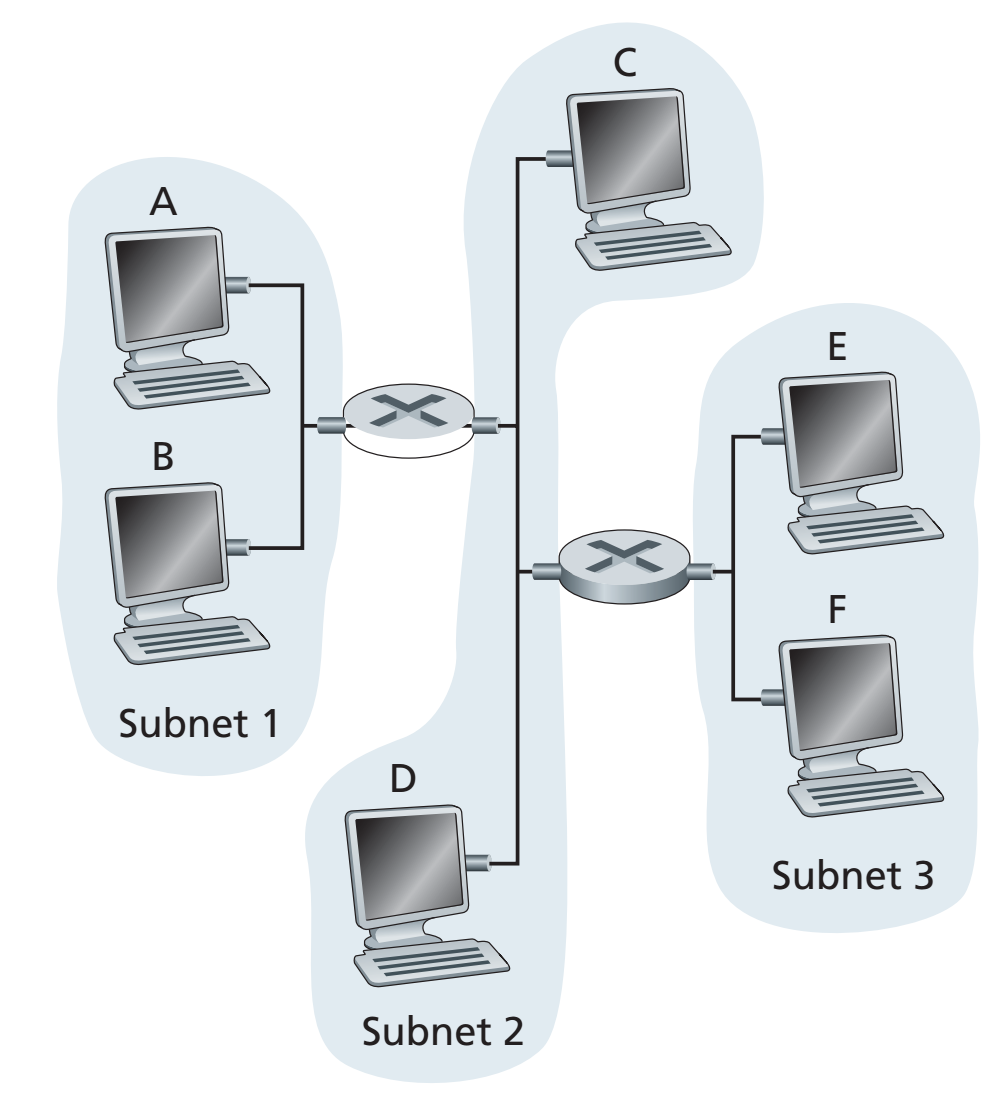
\includegraphics[width=0.5\textwidth,height=\textheight]{Figuras/fig3.png}

\begin{enumerate}
\def\labelenumi{\alph{enumi}.}
\tightlist
\item
  Atribua endereços IP a todas as interfaces. Para a Sub-rede 1, use
  endereços do formato 192.168.1.xxx; para a Sub-rede 2, use endereços
  do formato 192.168.2.xxx; e para a Sub-rede 3 use endereços do formato
  192.168.3.xxx.
\item
  Atribua endereços MAC a todos os adaptadores.
\item
  Considere enviar um datagrama IP do Host E para o Host B. Suponha que
  todas as tabelas ARP estejam atualizadas. Enumere todas as etapas.
\item
  Repita (c), agora assumindo que a tabela ARP no host de envio esteja
  vazia (e as outras tabelas estejam atualizadas).
\end{enumerate}

\begin{enumerate}
\def\labelenumi{\arabic{enumi}.}
\setcounter{enumi}{7}
\item
  Qual a diferença entre hub, switch e roteador? Em quais situações a
  utilização de cada um é mais adequada?
\item
  Explique qual tipo de problema as VLANs podem resolver e especifique,
  em termos de hardware, os requisitos necessários para sua
  implementação.
\item
  O que são as portas trunk dos switchs nível 3?
\end{enumerate}

\hypertarget{lista-de-exercuxedcios-sobre-scapy}{%
\subsection{Lista de Exercícios sobre
Scapy}\label{lista-de-exercuxedcios-sobre-scapy}}

\justify

Cada questão aborda um conceito fundamental da camada de enlace
utilizando o Scapy:

\begin{enumerate}
\def\labelenumi{\arabic{enumi}.}
\tightlist
\item
  Criação de Pacotes com Camada de Enlace:
\end{enumerate}

Utilizando o Scapy, crie um pacote que inclua a camada de enlace
\textbf{Ether} com:

\begin{itemize}
\tightlist
\item
  Endereço MAC de origem: \texttt{00:11:22:33:44:55}
\item
  Endereço MAC de destino: \texttt{FF:FF:FF:FF:FF:FF}
\item
  Uma camada IP com destino \texttt{192.168.1.1}.
\end{itemize}

Exiba os detalhes do pacote criado com o método \texttt{show()}.

\begin{enumerate}
\def\labelenumi{\arabic{enumi}.}
\setcounter{enumi}{1}
\tightlist
\item
  Envio de Pacotes ARP:
\end{enumerate}

Crie e envie um pacote ARP na camada de enlace que realize uma
solicitação de resolução de endereço (gratuitous ARP). Configure o MAC
de destino como \texttt{FF:FF:FF:FF:FF:FF} e o IP de destino como
\texttt{192.168.0.1}. Use o método \texttt{sendp()} para enviá-lo.

\begin{enumerate}
\def\labelenumi{\arabic{enumi}.}
\setcounter{enumi}{2}
\tightlist
\item
  Inspeção de Campos na Camada Ether:
\end{enumerate}

Liste e explique brevemente os campos disponíveis na camada de enlace
\textbf{Ether} utilizando o Scapy. Mostre também um exemplo de como
verificar esses campos programaticamente.

\begin{enumerate}
\def\labelenumi{\arabic{enumi}.}
\setcounter{enumi}{3}
\tightlist
\item
  Captura de Pacotes ARP:
\end{enumerate}

Utilize o Scapy para capturar 5 pacotes ARP na camada de enlace. Filtre
os pacotes capturados para exibir somente os endereços IP de origem
(\texttt{psrc}) e os endereços MAC de origem (\texttt{hwsrc}).
